%package list
\documentclass{article}
\usepackage[top=3cm, bottom=3cm, outer=3cm, inner=3cm]{geometry}
\usepackage{graphicx}
\usepackage{subfigure} % subfiguras
\usepackage{url}
%\usepackage{cite}
\usepackage{hyperref}
\usepackage{array}
\usepackage{multicol}
\newcolumntype{x}[1]{>{\centering\arraybackslash\hspace{0pt}}p{#1}}
%\usepackage{natbib}
\usepackage{pdfpages}
\usepackage{multirow}
\usepackage{float}
\usepackage[normalem]{ulem}
\useunder{\uline}{\ul}{}

\usepackage{listings}
\usepackage{xcolor}
\usepackage{algorithm,algorithmic}


\definecolor{codegreen}{rgb}{0,0.6,0}
\definecolor{codegray}{rgb}{0.5,0.5,0.5}
\definecolor{codepurple}{rgb}{0.58,0,0.82}
\definecolor{backcolour}{rgb}{0.95,0.95,0.92}

\lstdefinestyle{style_code}{
    backgroundcolor=\color{backcolour},   
    commentstyle=\color{codegreen},
    keywordstyle=\color{magenta},
    numberstyle=\tiny\color{codegray},
    stringstyle=\color{codepurple},
    basicstyle=\ttfamily\footnotesize,
    breakatwhitespace=false,         
    breaklines=true,                 
    captionpos=b,                    
    keepspaces=true,                 
    numbers=left,                    
    numbersep=5pt,                  
    showspaces=false,                
    showstringspaces=false,
    showtabs=false,                  
    tabsize=2
}

\lstset{style=style_code}


%%%%%%%%%%%%%%%%%%%%%%%%%%%%%%%%%%%%%%%%%%%%%%%%%%%%%%%%%%%%%%%%%%%%%%%%%%%%
%%%%%%%%%%%%%%%%%%%%%%%%%%%%%%%%%%%%%%%%%%%%%%%%%%%%%%%%%%%%%%%%%%%%%%%%%%%%
\newcommand{\csemail}{vmachacaa@unsa.edu.pe}
\newcommand{\csdocente}{Vicente Machaca Arceda}
\newcommand{\cscurso}{Estructura de Datos y Algoritmos}
\newcommand{\csuniversidad}{Universidad Nacional de San Agustín}
\newcommand{\csescuela}{Maestría en Ciencia de la Computación}
\newcommand{\cspracnr}{01}
\newcommand{\cstema}{Algoritmos de Ordenamiento}
%%%%%%%%%%%%%%%%%%%%%%%%%%%%%%%%%%%%%%%%%%%%%%%%%%%%%%%%%%%%%%%%%%%%%%%%%%%%
%%%%%%%%%%%%%%%%%%%%%%%%%%%%%%%%%%%%%%%%%%%%%%%%%%%%%%%%%%%%%%%%%%%%%%%%%%%%

\usepackage[english,spanish]{babel}
\usepackage[utf8]{inputenc}
\AtBeginDocument{\selectlanguage{spanish}}
\renewcommand{\figurename}{Figura}
\renewcommand{\refname}{Referencias}
\renewcommand{\tablename}{Tabla} %esto no funciona cuando se usa babel
\AtBeginDocument{%
	\renewcommand\tablename{Tabla}
}


\usepackage{fancyhdr}
\pagestyle{fancy}
\fancyhf{}
\setlength{\headheight}{30pt}
\renewcommand{\headrulewidth}{1pt}
\renewcommand{\footrulewidth}{1pt}
\fancyhead[L]{\raisebox{-0.2\height}{
\includegraphics[width=3cm]{img/logo_unsa}}}
\fancyhead[C]{}
\fancyhead[R]{\fontsize{7}{7}\selectfont	\csuniversidad \\ \csescuela \\ \textbf{\cscurso} }
\fancyfoot[L]{MSc. Vicente Machaca}
\fancyfoot[C]{\cscurso}
\fancyfoot[R]{Página \thepage}


\begin{document}
	
	\vspace*{10px}
	
	\begin{center}	
		\fontsize{17}{17} \textbf{ Práctica \cspracnr}
	\end{center}
	%\centerline{\textbf{\underline{\Large Título: Informe de revisión del estado del arte}}}
	%\vspace*{0.5cm}
	

	\begin{table}[h]
		\begin{tabular}{|x{4.7cm}|x{4.8cm}|x{4.8cm}|}
			\hline 
			\textbf{DOCENTE} & \textbf{CARRERA}  & \textbf{CURSO}   \\
			\hline 
			\csdocente & \csescuela & \cscurso    \\
			\hline 
		\end{tabular}
	\end{table}	
	
	
	\begin{table}[h]
		\begin{tabular}{|x{4.7cm}|x{4.8cm}|x{4.8cm}|}
			\hline 
			\textbf{PRÁCTICA} & \textbf{TEMA}  & \textbf{DURACIÓN}   \\
			\hline 
			\cspracnr & \cstema & 3 horas   \\
			\hline 
		\end{tabular}
	\end{table}
	
	
	\section{Datos de los estudiantes}
	\begin{itemize}
		\item Grupo: 9
		\item Integrantes: 
		\begin{itemize}
			\item Abarca Murillo, Jhonatan Piero
			\item Apari Pinto, Christian Timoteo
			\item Suca Velando, Christian Anthony
			\item Vargas Zuni, Arturo
		\end{itemize}
		\item Repositorio: \url{https://github.com/jabarcamu/EDA_Practica1}
	\end{itemize}
	

	
	\section{Ejercicios}\label{sec:ejercicios}
	
		\subsection{Preparación de Datos}
		
    		La generación de datos se realizó de la siguiente manera:
    		\begin{itemize}
    		    \item Por medio las librerías de generación de números aleatorios y ademas de la libreria de escritura para archivos .txt de inicio con la generación de los archivos
    		    \item Cada Archivo tiene el nombre de la cantidad de números generados aleatoriamente.
    		    \item Cada archivo contiene 100, 500, 1000, 2000, 3000, ..., 10000, 20000, 30000, ..., 1000000.
    		    \item El resultado final se utilizará para ordenar a cada uno de los números generados en cada archivo creado, estos archivos estarán en la carpeta del repositorio donde se alojarán y serán utilizados para la segunda parte de la práctica.
    		\end{itemize}
    		
    		Los archivos generados se guardarán con la denominación ejemplo\textunderscore$<$número\textunderscore iteraciones$>$ en la misma ruta del archivo donde se ejecuta el codigo en la carpeta ``generatedTestData". El resultado se muestra en la figura \ref{fig:prep_datos_fig1}.
    		
    		
    		\begin{figure}[H]
				\centering
				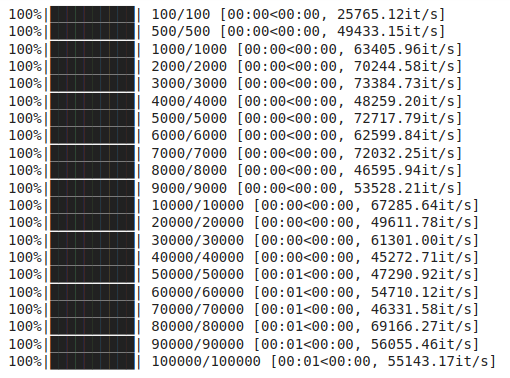
\includegraphics[scale=0.40]{img/1_preparacion_datos.png}
				\caption{Archivos generados}
				\label{fig:prep_datos_fig1}
			\end{figure}
			
			Para la creacion de los archivos se requeria iterar sobre un mismo archivo el cual se realiza mediante el uso de la libreria numpy tomando los rangos pedidos en la práctica. Sobre la lista generada se declara la ruta de generacion del archivo resultante y sobre la misma iterar la lista de numeros generados anteriormente.
			\\
			Ya estando dentro de cada iteracion mediante el uso de random de la libreria numpy se realiza la generacion de numeros segun sea el turno de iteracion (desde 100 hasta 100000), tal cual como se puede observa en el código mostrado.
    		
    		\lstinputlisting[language=Python, caption=generatedFiles.py]{code/generatedFiles.py}
		
		\subsection{Implementaci\'{o}n de algoritmos}
		    La implementaci\'{o}n de todos los algoritmos que presentaremos a continuación estan implementados en los lenguajes C++ y Python.
		    
		    
		        \subsubsection{Bubble sort} 
		        Según la definición del libro \cite{CLRS2009} el algoritmo Bubble Sort tiene la siguiente estructura, concepto y pseudocodigo:
		        
		            \begin{flushleft}
    		            \textbf{Input:} Un arreglo de \textit{n} números enteros positivos $<a_1,a_2,...,a_n>$ , un arreglo de \textit{n} números enteros positivos inicializados en 0 para almacenar el resultado $<0_1,0_2,...,0_n>$ y el máximo valor del arreglo \textit{n}  \\
    		            \textbf{Output:} Un arreglo ordenado $<a'_1 \leq a'_2 \leq ... \leq a'_n>$
		            \end{flushleft}
		            
		            El procedimiento de ejecución comienza con un arreglo de números enteros distribuidos de forma aleatoria, los cuales deben ser ordenados con una búsqueda secuencial sobre los elementos ya procesados, esto consiste en recorrer una y otra vez los elementos del arreglo que ya fueron ordenados, encontrar una posicion especifica e intercambiar con el elemento seleccinoado, para este procedimiento utilizaremos una variable temporal que realizará el intercambio de valores, a continuación se muestra un pseudocódigo de la ejecución del algoritmo.
		            
		            \begin{algorithm}[H]
                        \begin{algorithmic}[1]
                            \FOR{$i \gets 1$ to $N$}
                                \FOR{$j \gets i+1$ to $N$}
                                    \IF{$A[j] < A[i]$}
                                        \STATE $temp \gets A[i]$
                                        \STATE $A[i] \gets A[j];$ 
                                        \STATE $A[j] \gets temp;$
                                    \ENDIF    
                                \ENDFOR
                            \ENDFOR
                        \end{algorithmic}
                        \caption{BUBBLE-SORT(A)}
                        \label{alg:bubble-sort}
                    \end{algorithm}
                    
                    \begin{enumerate}
                        \item \textbf{An\'{a}lisis}\\
                            La complejidad computacional del algoritmo es $O(n^{2})$, en el peor y mejor caso. Siendo \textit{n} la cantidad de elementos a ordenar.
                            
                        \item \textbf{Implementaci\'{o}n C++}
                
                        \lstinputlisting[language=C++, firstline=1, lastline=12, caption=BubbleSort.cpp]{code/bubble_sort_code.cpp}
                        
                        \item \textbf{Implementaci\'{o}n Python}\\
                
                        \lstinputlisting[language=Python, firstline=1, lastline=7, caption=BubbleSort.py]{code/bubble_sort_code.py}
                        
                    \end{enumerate}
		            
		        \subsubsection{Counting Sort}
		            \begin{flushleft}
    		            \textbf{Input:} Un arreglo de \textit{n} números enteros positivos $<a_1,a_2,...,a_n>$ , un arreglo de \textit{n} números enteros positivos inicializados en 0 para almacenar el resultado $<0_1,0_2,...,0_n>$ y el máximo valor del arreglo \textit{n}  \\
    		            \textbf{Output:} Un arreglo ordenado $<a'_1 \leq a'_2 \leq ... \leq a'_n>$
		            \end{flushleft}
		            
		         
		            \begin{algorithm}[H]
                        \begin{algorithmic}[1]
                            \FOR{$i \gets 0$ to $K$}
                                \STATE $C[i] \gets 0$
                            \ENDFOR
                            \FOR{$j \gets 1$ to $length[A]$}
                                \STATE $C[A[j]] \gets C[A[j]] + 1$
                            \ENDFOR
                            \FOR{$i \gets 1$ to $k$}
                                \STATE $C[i] \gets C[i] + C[i - 1]$
                            \ENDFOR
                            \FOR{$j \gets length[A]$ to $1$}
                                \STATE $B[C[A[j]]] \gets A[j]$
                                \STATE $C[A[j]] \gets C[A[j]]-1$
                            \ENDFOR
                        \end{algorithmic}
                        \caption{COUNTING-SORT(A,B,k)}
                        \label{alg:counting-sort}
                    \end{algorithm}
                    El algoritmo countingsort fue propuesto por Harold H. Seward en 1954. Permite ordenar números sin necesidad de realizar comparaciones, usando un contador para almacenar los valores repetidos del arreglo.
                    Los pasos del algoritmo son:
    		        \begin{itemize}
    		            \item Obtener el valor máximo del arreglo.
    		            \item Crear un arreglo temporal del mismo tamaño del valor máximo, e inicializarlo en 0.
    		            \item Recorrer el arreglo principal e incrementar el contador del arreglo temporal por cada elemento del arreglo hallado.
    		            \item Recorrer el arreglo principal, y conjuntamente con el arreglo temporal, ubicar los elementos en su posición correcta en base a la cantidad de valores del contador.
    		        \end{itemize}
    		        \begin{figure}[H]
        				\centering
        				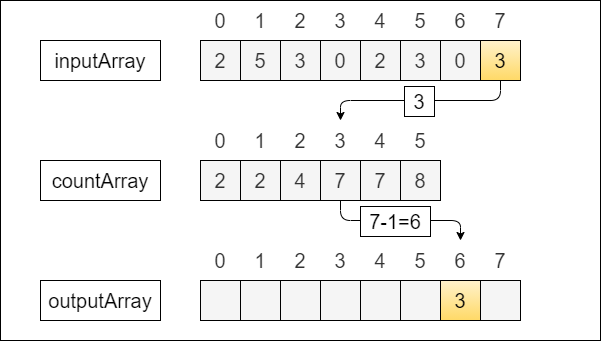
\includegraphics[scale=0.40]{img/countingsort.png}
        				\caption{Counting Sort en funcionamiento}
        				\label{fig:counting_sort_img1}
        			\end{figure}
                    
                    \begin{enumerate}
                        \item \textbf{An\'{a}lisis}\\
                            La complejidad computacional del algoritmo es $O(n+k)$, en el peor y mejor caso. Siendo \textit{n} la cantidad de elementos a ordenar y \textit{k} el tamaño de arreglo auxiliar(memoria adicional).
                        \begin{itemize}
        		            \item Se puede adaptar tanto a números decimales, así como a caracteres, pero con un costo adicional.
        		            \item La mayor limitación del algoritmo lo provoca la cantidad de memoria extra necesaria para realizar el algoritmo, dicho proceso se da cuando el rango entre el mayor y menor valor del arreglo son muy grandes.
        		        \end{itemize}
                            
                            \item \textbf{Implementaci\'{o}n C++}
                    
                            \lstinputlisting[language=C++, firstline=19, lastline=59, caption=countingSort.cpp]{code/counting.cpp}
                            
                            \item \textbf{Implementaci\'{o}n Python}\\
                    
                            \lstinputlisting[language=Python, firstline=11, lastline=46, caption=countingSort.py]{code/counting.py}
                        
                    \end{enumerate}
		        
		        \subsubsection{Heap Sort}
		        
		            \begin{flushleft}
    		            \textbf{Input:} Un arreglo de \textit{n} elementos  $<a_1,a_2,...,a_n>$ que pueden ser ordenado por su clave (car\'{a}cter, n\'{u}mero)\\
    		            \textbf{Output:} Un arreglo ordenado $<a'_1 \leq a'_2 \leq ... \leq a'_n>$
		            \end{flushleft}
		            
    		        El algoritmo de heapsort fue creado por los autores J. Williams y refinado por R.W Floyd en el año 1964, se basa en un almacenamiento de datos conocido como Heap, su representación de la ra\'{i}z es dado por $A[1]$ y dado cualquier \'{i}ndice $i$ de nodo se puede obtener:
    		        \begin{itemize}
    		            \item padre $Parent(i) \leftarrow \lfloor i/2 \rfloor$
    		            \item hijo izquierdo $Left(i) \leftarrow 2i$
    		            \item hijo derecho $Right(i) \leftarrow 2i + 1$
    		        \end{itemize}
    		        
    		        Esta estructura basada en un \'{a}rbol binario mantiene una propiedad o invariante de que en cada nivel cualquier nodo sea siempre mayor a sus hijos $A[Parent(i)] \geq A[i]$, como se observa en la figura \ref{fig:heap_repr}.
    		         
    		        \begin{figure}[H]
    		            \centering	 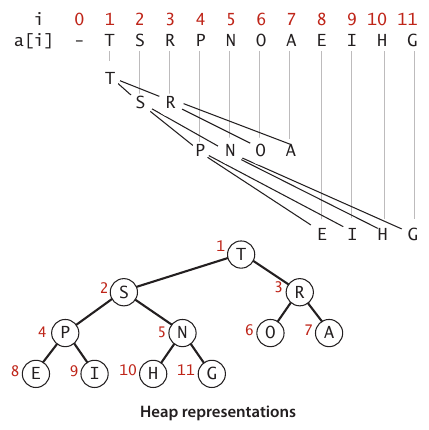
\includegraphics[scale=0.40]{img/heap_repre.png}
                        \caption{Representaci\'{o}n de un Heap como arbol Binario \cite{Algorithms}}
                        \label{fig:heap_repr}
                    \end{figure}
                    			
                    Adem\'{a}s  se usan operaciones definidas en una cola de prioridad para elaborar un ordenamiento conocido como heapsort, tales operaciones como Swim y Sink son fundamentales para mantener las propiedades general o invariante. La operaci\'{o}n Swim se encarga de preguntar por los hijos si son mayores a sus padres, intercambiando siempre aquellos nodos que no cumplan esta condici\'{o}n y recursivamente ser llamada hasta llegar a la ra\'{i}z, con respecto a Sink es lo inverso, pregunta por los padres si son menores a sus hijos, si es as\'{i}, va intercambiando los nodos para que se cumpla la invariante, progresivamente hacia abajo hasta llegar a un nodo hoja, esta funci\'{o}n es la que se usa en el heapsort.
    		            
    		        Para el ordenamiento Heapsort se requieren dos principales tareas, el ordenamiento por heap Build-Max-Heap y el ordenamiento hacia abajo SortDown aplicando Max-Heapify.
    		            
    		        El Build-Max-Heap, el principal objetivo es hacer cumplir la invariante, el cual es que todo nodo padre sea mayor a sus nodos hijo, la construcci\'{o}n del max-heap har\'{a} que los elementos mas grandes estén al inicio del array y los elementos menos grandes muy cerca del primer elemento, esto requiere aplicar comparaciones del nodo actual con sus respectivos hijos y saber si el nodo siempre ser\'{a} mayor a sus hijos, en caso de no serlo se producir\'{a} el intercambio y recursivamente se ayudar\'{a} de la funci\'{o}n Max-Heapify haciendo la propagaci\'{o}n hacia abajo. Adem\'{a}s no requiere que se cubra todo el array ya que los nodos hoja al ser un Heap de tama\~{n}o uno no requiere realizar un proceso de Max-Heapify. Es as\'{i} que a lo mucho el costo de realizar el Build-Max-Heap es un coste lineal O(n).
    		            
    		        El seudoc\'{o}digo para el primer proceso Build-Max-Heap es el siguiente:
    		            
    		        \begin{algorithm}[H]
                        \begin{algorithmic}[1]
                            \STATE $heap-size[A] \leftarrow length[A]$
                            \FOR{$i \leftarrow \lfloor length[A]/2 \rfloor$ to $1$}
                                \STATE $Max-Heapify(A,i)$
                            \ENDFOR
                        \end{algorithmic}
                        \caption{Build-Max-Heap(A)}
                        \label{alg:build-max-heap}
                    \end{algorithm}
                        
                    De acuerdo al seudoc\'{o}digo \ref{alg:build-max-heap} el tamaño de heap comenzar\'{a} con todo los items del arreglo $A$ y a partir de la mitad de los elementos del array hacia el primer elemento son considerados nodos intermedios del \'{a}rbol y la propia ra\'{i}z, sin considerar los nodos hoja o terminales ya que estos cumplen la propiedad de invarianza, conforme se va iterando se aplica la funci\'{o}n Max-Heapify, (propagaci\'{o}n hacia abajo) pero que siempre ir\'{a} cambiando el nodo evaluado, desde los nodos intermedios hasta llegar a la ra\'{i}z.
                        
                    Max-Heapify se aplica al nodo actual que se esta evaluando y recursivamente eval\'{u}a los nodos hacia abajo (Sink). En otra palabras se hace cumplir la propiedad por subHeap.
                        
                    El segundo proceso, es el SortDown aplicando Max-Heapify quien se encarga principalmente de hacer cumplir la invariante, cuando se eval\'{u}a Max-Heapify puede darse el caso de no cumplir la invariante y viole la propiedad max-heap por ese motivo el valor actual $A[i]$ navegar\'{a} hacia abajo (Sink), as\'{i} el sub\'{a}rbol con ra\'{i}z $i$ se convertir\'{a} en un max-heap o sub-mont\'{i}culo.
                        
                    \begin{algorithm}[H]
                        \begin{algorithmic}[1]
                            \STATE $l \leftarrow LEFT(i)$
                            \STATE $r \leftarrow RIGHT(i)$
                            \IF{ $l \leq heap-size[A]  \AND  A[l] > A[i]$}
                                \STATE $largest \leftarrow l$
                            \ELSE
                                \STATE $largest \leftarrow i$
                            \ENDIF
                            \IF{ $r \leq heap-size[A] and A[r] > A[largest]$}
                                \STATE $largest \leftarrow r$
                            \ENDIF
                            \IF{ $largest \neq i$}
                                \STATE $exchange A[i] \leftrightarrow A[largest]$
                                \STATE $Max-Heapify(A, largest)$
                            \ENDIF
                        \end{algorithmic}
                        \caption{Max-Heapify(A,i)}
                        \label{alg:max-heapify}
                    \end{algorithm}
    		         
    		        Es as\'{i} que el algoritmo de heapsort usa primero el Build-Max-Heap para hacer cumplir la invariante en todos los nodos $A[1..n]$ donde $n=length[A]$, y hacer que el primero elemento del array sea mayor a todos sus descendientes, dando la posibilidad de intercambiar el elemento final con la ra\'{i}z haciendo que este elemento ya se encuentre ordenado por ser el mayor de los elementos $A[1]$. Este elemento queda ya descartado del heap $heap-size[A] - 1$.
    		         
    		        Sin embargo este elemento intercambiado se tendr\'{a} que evaluar su propiedad de Max-Heap por lo cual se aplicar\'{a} la funci\'{o}n Max-Heapify sobre el primer elemento $Max-Heapify(A,1)$ y propagar hacia abajo, hasta que se cumpla la invariante.
    		         
    		        Esto se har\'{a} iterando desde el \'{u}ltimo elemento $length[A]$ hasta llegar al segundo item dejando espacio para el intercambio con el primer elemento $A[1]$. El completo algoritmo de heapsort es dado en el seudoc\'{o}digo \ref{alg:heapsort}
		         
		            \begin{algorithm}[H]
                        \begin{algorithmic}[1]
                            \STATE $BUILD-MAX-HEAP(A)$
                            \FOR{$i \leftarrow length[A]$ downto $2$}
                                \STATE exchange $A[1] \leftrightarrow A[i]$
                                \STATE $heap-size[A] \leftarrow heapsize[A]-1$
                                \STATE $MAX-HEAPIFY(A,1)$
                            \ENDFOR
                        \end{algorithmic}
                        \caption{Heapsort(A)}
                        \label{alg:heapsort}
                    \end{algorithm}
		        
		            En la siguiente figura se puede ver el proceso del Heapsort  \ref{fig:heap_trace} tanto para el proceso de construcci\'{o}n o BUILD-MAX-HEAP y para el proceso de SortDown con la aplicaci\'{o}n de Max-Heapify por cada nodo intermedio.
		            
		            \begin{figure}[H]
    		            \centering	 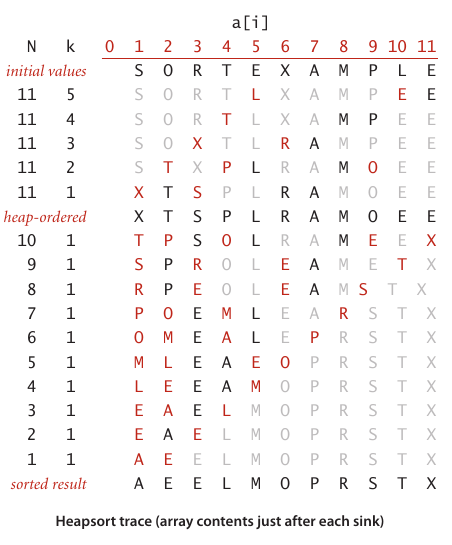
\includegraphics[scale=0.40]{img/heapsort_trace.png}
                        \caption{Aplicaci\'{o}n del algoritmo Heapsort: Construcción y SortDown \cite{Algorithms}}
                        \label{fig:heap_trace}
                    \end{figure}
                    
                    \begin{enumerate}
                        \item \textbf{An\'{a}lisis}\\
                            El procedimiento de Heapsort toma un tiempo de O(nlgn).
                            El Build-Max-Heap toma un tiempo lineal O(n) y es absorbido por el coste del SortDown el cual es mayor, el coste de Build-Max-Heap es lineal ya que es una cota ajustada por el hecho de que la llamada a Max-Heapify interna, va relacionada con la altura de los mont\'{i}culos y multiplicado por el n\'{u}mero de nodos dados en un nivel particular, esto sumado por cada nivel de la construcción en el \'{a}rbol, da un orden lineal O(n).
                            
                            En cuanto al proceso de SortDown se realizar n-1 
                            llamadas de Max-Heapify interno el cual por si solo tiene un coste de O(lgn), en este caso Max-Heapify toma un coste de acuerdo a la altura del montículo. Es así que el coste total de el proceso de SortDown es O(nlgn) y es el coste del proceso de Heapsort.
                            
                        \item \textbf{Implementaci\'{o}n C++}
                    
                            \lstinputlisting[language=C++, firstline=10, lastline=36, caption=heapsort.cpp]{code/heapsort.cpp}
                            
                            \item \textbf{Implementaci\'{o}n Python}\\
                    
                            \lstinputlisting[language=Python, firstline=33, lastline=54, caption=heapsort.py]{code/heapsort.py}
                    \end{enumerate}
		         
		         
		         \subsubsection{Insertion Sort}
		         
		            Tomando lo que define \cite{CLRS2009} como parte de su primer algoritmo de ordenamiento:
		            
		            \begin{flushleft}
    		            \textbf{Input:} Una secuencia de \textit{n} números $<a_1,a_2,...,a_n>$ \\
    		            \textbf{Output:} Una permutación(reordenar) $<a'_1,a'_2,...,a'_n>$ de la secuencia 
    		            de entrada tal que $<a'_1 \leq a'_2 \leq ... \leq a'_n>$
		            \end{flushleft}
		            
		            Inicia con una lista vacia de una cantidad de elementos. Algo similar a como se ordena una mano de cartas o naipes. Inicia con una mano izquierda vacia y cartas boca abajo sobre la mesa. Se remueve una carta de la mesa al mismo tiempo que se inserta una en la mano y se inserta en la posicion correcta de la mano izquierda. Para encontrar una correcta posicion de la carta, comparemoslo con cada una de las cartas ya en mano, de izquierda a derecha. En todas las veces, las cartas que se mantuvieron en la mano izquierda estan ordenadas ya que estas cartas, fueron originalmente, las que estuvieron encima de la mesa.
		            \\
		            El siguiente pseudocódigo \ref{alg:insertion-sort}, que toma como parametro una lista $A[n]$, con $n$ como el tamaño de la lista a ser ordenada. El índice $i$ indica la ``carta actual" siendo insertada en la mano. Al principio de cada iteracion del bucle $for$, el cual esta indexado con $i$, el subarray a ordenar corresponde a $A[1...i-1]$, la mano actualmente ordenada, y el array sobrante $A[i+1..n]$ corresponde a la pila de cartas aun en la mesa. El hecho es que los elementos $A[1...i-1]$ son los elementos originalmente en la posicion 1 a traves de $i-1$, pero ahora ordenado, conocido como bucle invariante, al inicio de cada iteracion del bucle $for$ se ordena por llegada \cite{CLRS2009}.
		         
		            \begin{algorithm}[H]
                        \begin{algorithmic}[1]
                            \FOR{$i \gets 1$ to $N$}
                                \STATE $key \gets A[i]$
                                \STATE $j \gets i-1$
                                \WHILE{$j>=0$ and $A[j] > key$}
                                    \STATE $A[j + 1] \gets A[j]$ 
                                    \STATE $j \gets j - 1$
                                \ENDWHILE
                                \STATE $A[j + 1] \gets key$
                            \ENDFOR
                        \end{algorithmic}
                        \caption{INSERTION-SORT(A)}
                        \label{alg:insertion-sort}
                    \end{algorithm}
                    
                    \begin{enumerate}
                        \item \textbf{An\'{a}lisis}\\
                            En el mejor caso de los $n$ items estan en sus respectivos lugares ordenados, entonces Insertion Sort tomará un tiempo lineal o $O(n)$. Esto podría parecer un punto trivial, ya que frecuentemente no se encuentra una lista totalmente ordenda, pero si es importante saberlo ya que es un algoritmo al cual se le puede analizar su mejor caso.
                            \\
                            En el mundo real, Insertion Sort para datos parcialmente ordenados, podria ser un algoritmo efectivo de usar. La eficiencia de Insertion sort se incrementa cuando duplicamos los items.
                            \\
                            Desafortunadamente tomando el peor caso en que todos items se transpongan en su posición a la inversa, Insertion Sort requiere $O(n^2)$ (tiempo cuadrático).
                            
                            \begin{figure}[H]
                				\centering
                				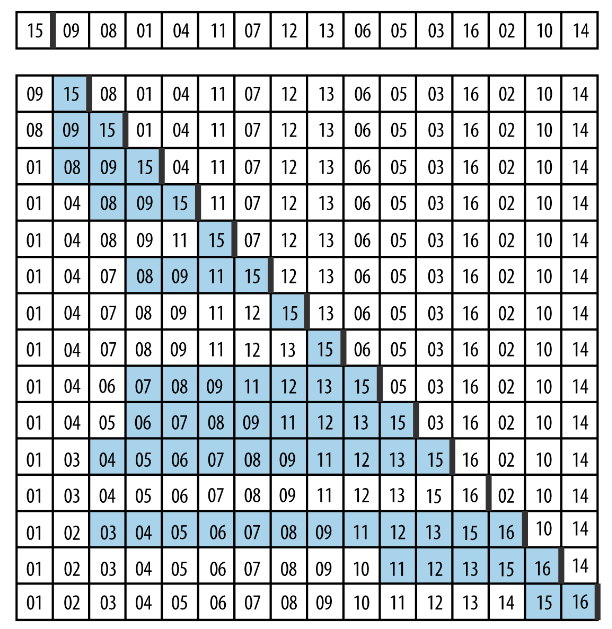
\includegraphics[scale=0.40]{img/insertion_sort_image1.PNG}
                				\caption{Insertion Sort en ejecución sobre una lista pequeña \cite{Heineman2008}}
                				\label{fig:insertion_sort_img1}
                			\end{figure}
                            
                            Insertion Sort opera ineficientemente por valor de la data debido a la cantidad de memoria que debe intercambiarse cuando toma espacio para un nuevo valor.
                            
                            \item \textbf{Implementaci\'{o}n C++}
                    
                            \lstinputlisting[language=C++, firstline=11, lastline=33, caption=insertionSort.cpp]{code/insertion.cpp}
                            
                            \item \textbf{Implementaci\'{o}n Python}\\
                    
                            \lstinputlisting[language=Python, firstline=8, lastline=23, caption=insertionSort.py]{code/insertion.py}
                        
                    \end{enumerate}
		         
		         \subsubsection{Merge Sort}
		         
		            \begin{flushleft}
    		            \textbf{Input:} Un arreglo de \textit{n} números enteros positivos $<a_1,a_2,...,a_n>$ , un valor inferior \textit{p} y un valor superior \textit{r}  \\
    		            \textbf{Output:} Un arreglo ordenado $<a'_1 \leq a'_2 \leq ... \leq a'_n>$
		            \end{flushleft}
		            
		         
		            \begin{algorithm}[H]
                        \begin{algorithmic}[1]
                                \IF {$r > p$} 
                                    \STATE $m \gets p + (r-p)/2$ 
                                    \STATE CALL mergeSort(A,p,m)
                                    \STATE CALL mergeSort(A,m+1,r)
                                    \STATE CALL merge(A,p,m,r)
                                \ENDIF
                        \end{algorithmic}
                        \caption{MERGE-SORT(A,p,r)}
                        \label{alg:merge-sort}
                    \end{algorithm}
                    
                    \begin{algorithm}[H]
                        \begin{algorithmic}[1]
                            \STATE $n1 \gets q-p+1$
                            \STATE $n2 \gets r-q$
                            \STATE create arrays L[1..n1+1] and R[1..n2+1]
                            \FOR{$i \gets 1$ to $n1$}
                                \STATE $L[i] \gets A[p+i-1]$
                            \ENDFOR
                            \FOR{$j \gets 1$ to $n2$}
                                \STATE $R[j] \gets A[q+j]$
                            \ENDFOR
                            \STATE $i \gets 1$
                            \STATE $j \gets 1$
                            \STATE $k \gets l$
                            \WHILE{$i < n1$ and $ j < n2$}
                                \IF {$L[i] <= R[j]$} 
                                    \STATE $A[k] \gets L[i]$ 
                                    \STATE $i \gets i + 1$ 
                                \ELSE
                                    \STATE $A[k] \gets R[j]$ 
                                    \STATE $j \gets j + 1$
                                \ENDIF
                                \STATE $k = k + 1;$
                            \ENDWHILE
                            \WHILE{$i < n1$}
                                \STATE $A[k] = L[i]$
                                \STATE $i = i + 1;$
                                \STATE $k = k + 1;$
                            \ENDWHILE
                            \WHILE{$j < n2$}
                                \STATE $A[k] = R[j]$
                                \STATE $j = j + 1;$
                                \STATE $k = k + 1;$
                            \ENDWHILE
                        \end{algorithmic}
                        \caption{MERGE(A,p,q,r)}
                        \label{alg:merge}
                    \end{algorithm}
                     Fue desarrollado en 1945, por Jhon Von Neumann. Este algoritmo recursivo se basa en la técnica divide y vencerás.
                    Los pasos del algoritmo son:
    		        \begin{itemize}
    		            \item Hallar el punto medio del arreglo.
    		            \item Dividir el arreglo no ordenado en dos subarreglos cuyo tamaño son aproximadamente la mitad del arreglo principal.
    		            \item Llamar recursivamente a cada subarreglo(izquierdo y derecho) hasta encontrar el arreglo contiene un solo elemento, el cual explícitamente indica que el arreglo ya esta ordenado.
    		            \item Iniciar el proceso de mezcla de subarreglos ordenados hasta completar la unión del arreglo inicial.
    		        \end{itemize}
    		        \begin{figure}[H]
        				\centering
        				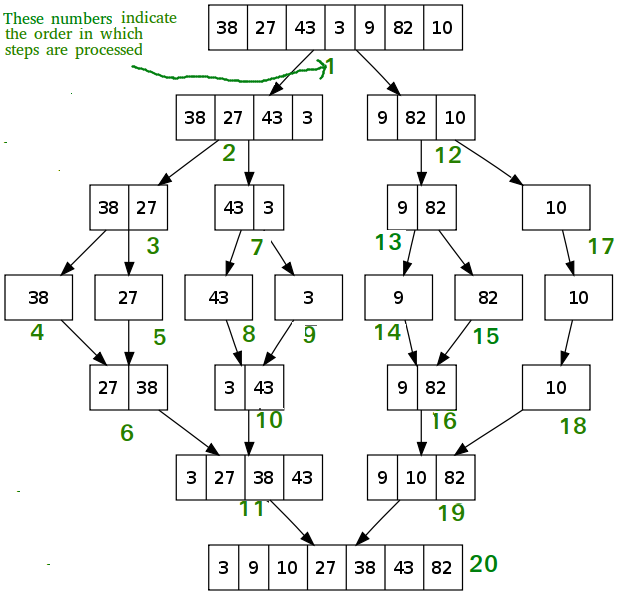
\includegraphics[scale=0.40]{img/mergesort.png}
        				\caption{Merge Sort en funcionamiento}
        				\label{fig:merge_sort_img1}
        			\end{figure}
                    \begin{enumerate}
                        \item \textbf{An\'{a}lisis}\\
                            La complejidad computacional del algoritmo en el mejor caso, en el caso promedio y en el peor de los caso es siempre $O(n log n)$. 
                            \begin{itemize}
            		            \item El ordenamiento no trabaja in situ, es decir que no realiza un cambio en el mismo arreglo directamente, sino que hace una copia antes de actualizar el arreglo.
            		            \item Para mezclar los dos subarreglos, ambos deberán estar ordenados.
            		            \item Mergesort requiere un espacio auxiliar $(n)$, en comparación con Heapsort que requiere un espacio de $(1)$
            		        \end{itemize}
                            \item \textbf{Implementaci\'{o}n C++}
                    
                            \lstinputlisting[language=C++, firstline=16, lastline=84, caption=mergeSort.cpp]{code/merge.cpp}
                            
                            \item \textbf{Implementaci\'{o}n Python}\\
                    
                            \lstinputlisting[language=Python, firstline=12, lastline=53, caption=mergeSort.py]{code/merge.py}
                        
                    \end{enumerate}
		         
		        \subsubsection{Quick Sort}
		        
    		        \begin{flushleft}
    		            \textbf{Input:} Un arreglo de \textit{n} elementos $<a_1,a_2,...,a_n>$ , posici\'{o}n inicial $p$, posici\'{o}n final $r \leftarrow length[A]$  \\
        		        
        		        \textbf{Output:} Un arreglo ordenado $<a'_1 \leq a'_2 \leq ... \leq a'_n>$
    		        \end{flushleft}
    		        
    		        El algoritmo de Quicksort fue inventado por el autor C.A.R. Hoare en 1960, este algoritmo es bastante eficiente y es garantizado el ordenamiento, en el peor caso con un orden de $O(n^2)$ y en el caso promedio $O(n\log(n))$, el ordenamiento es en lugar, solo requiere una pequeña pila adicional.
    		        La peque\~{n}a desventaja es que es bastante sensible al balance de los datos, si no estuvieran muy des-balanceados, es decir diversas tama\~{n}os del proceso de partici\'{o}n, podr\'{i}a ocasionar un tiempo considerable de orden $O(n^2)$
    		         
    		        QuickSort usa como base el concepto de divide y conquista, en este caso dado un array $A[p..r]$.
    		        
    		        \begin{itemize}
    		            \item Dividir: divide el arreglo en dos sub-arreglos de tama\~{n}o $A[p..q-1]$ y $A[q+1..r]$ donde $A[q]$ es mayor al primer sub-array y menor e igual al segundo sub-array. Computar q como parte de la partici\'{o}n
    		            \item Conquistar: Ordenar los subarrays por llamadas recursivas a quicksort
    		            \item Combinar: Desde que el ordenamiento es en el lugar no requiere la combinación. El array $A[p..r]$ estar\'{i}a ya ordenado.
    		        \end{itemize}
    		        
    		        En el siguiente seudoc\'{o}digo \ref{alg:quicksort} se da la implementaci\'{o}n del algoritmo quicksort.
    		        
    		        \begin{algorithm}[H]
                        \begin{algorithmic}[1]
                            \IF{$p<r$}
                                \STATE $q \leftarrow Partition(A,p,r)$
                                \STATE $QUICKSORT(A,p,q-1)$
                                \STATE $QUICKSORT(A,q+1,r)$
                            \ENDIF
                        \end{algorithmic}
                        \caption{QUICKSORT(A,p,r)}
                        \label{alg:quicksort}
                    \end{algorithm}
                    
                    El factor mas importante en el algoritmo de Quicksort es el proceso de partici\'{o}n , dado por el siguiente seudoc\'{o}digo \ref{alg:quick_partition}
                    
                    \begin{algorithm}[H]
                        \begin{algorithmic}[1]
                            \STATE $x \leftarrow A[r]$
                            \STATE $i \leftarrow p-1$
                            \FOR{$j \leftarrow p$ to $r-1$}
                                \IF{$A[j] \leq x$}
                                    \STATE $i \leftarrow i+1$
                                    \STATE $A[i] \leftrightarrow A[j]$
                                \ENDIF
                            \ENDFOR
                            \STATE exchange $A[i+1] \leftrightarrow A[r]$
                            \STATE return i+1
                        \end{algorithmic}
                        \caption{PARTITION(A,p,r)}
                        \label{alg:quick_partition}
                    \end{algorithm}
                    
                    El proceso de partici\'{o}n implica tomar el \'{u}ltimo elemento del array como pivote $x = A[r]$ el cual ser\'{a} el elemento que divida y genere los dos subarrays, en la inicializaci\'{o}n de los iteradores $i$ y $j$ se generan 4 regiones, la primer regi\'{o}n es la que contendrá los elementos menores al pivote, la segunda regi\'{o}n contendrá los elementos mayores e igual al pivote, la 3era regi\'{o}n es aquella que contendrá los elementos que serán comparados con el pivote y la \'{u}ltima regi\'{o}n es el que contiene el pivote.
                    
                    Por ello se satisface las siguientes propiedades aplicados a las l\'{i}neas del 3 al 6 en el seudoc\'{o}digo \ref{alg:quick_partition} y como se observa en la figura \ref{fig:quicksort_regions}
                    
                    \begin{figure}[H]
                        \centering
                        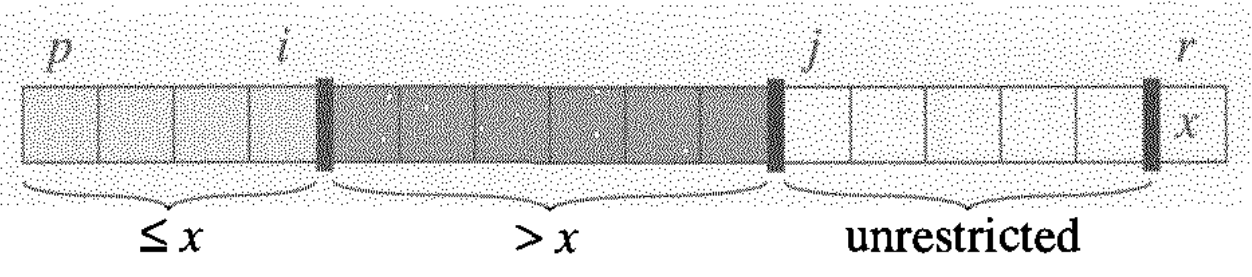
\includegraphics[scale=0.30]{img/quicksort_regions.png}
                		\caption{Regiones en el Partition}
                		\label{fig:quicksort_regions}
                	\end{figure}
                    
                    \begin{itemize}
                        \item Todos los elementos k que este entre $p$ y el \'{i}ndice $i$ son menores al pivote $x$.
                        \subitem IF $p \leq k \leq i$ THEN $A[k] \leq x$
                        
                        \item Todos los elementos k que est\'{e}n entre $i+1$ y $j-1$ son mayores al pivote $x$
                        \subitem IF $i+1 \leq k \leq j-1$ THEN $A[k] > x$
                        
                        \item Todos los elementos k entre $j+1$ y $r-1$ son elementos que deben ser comparados con el pivote $x$
                        \subitem IF $j+1 \leq k \leq r-1$ THEN $compare(A[k],x)$
                        
                        \item El elemento k ubicado en $r$, es el pivote actual $x$
                        \subitem IF $k=r$, then $A[k] = x$
                    \end{itemize}
                    
                    Una manera de ejemplificar los casos dados por la partici\'{o}n, dado en la siguiente figura \ref{fig:quick_cases_partition}, el primero es cuando $A[j] > x$, lo cual incrementa el j a\~{n}adiendolo al intervalo de los mas grandes que x, el segundo es cuando $A[j] <= x$, aquí el primer indice $i$ es incrementado con el objetivo de intercambiar uno de los items del intervalo grande por el elemento contenido en j (el menor al pivote) as\'{i} el intervalo de los m\'{a}s pequeños habr\'{a} ganado un item adicional. Posteriormente el j es incrementado para la siguiente item a comparar con el pivote. 
                    
                    \begin{figure}[H]
    		            \centering	 \subfigure[Caso para intervalo grande]{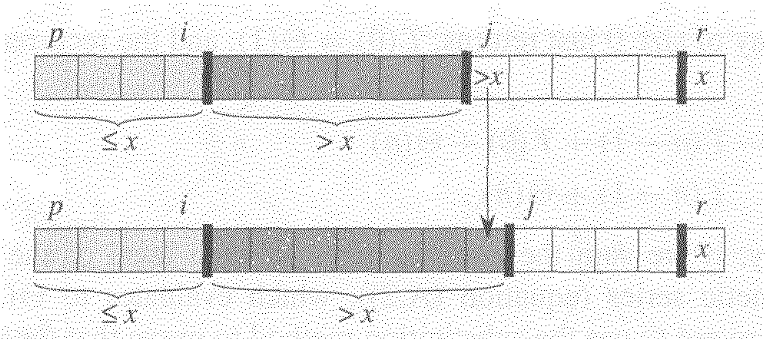
\includegraphics[scale=0.40]{img/partition_larger.png}}
    		            \subfigure[Caso para Intervalo peque\~{n}o]{ 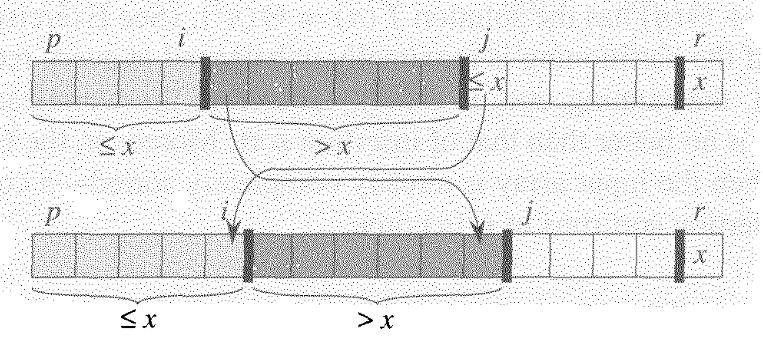
\includegraphics[scale=0.40]{img/partition_smaller.png}}
                        \caption{Casos dados en Partition \cite{Algorithms}}
                        \label{fig:quick_cases_partition}
                    \end{figure}
                    
                    Finalmente, el procedimiento de ordenamiento de Quicksort, donde se observa paso a paso la aplicaci\'{o}n de las particiones, dado en la figura \ref{fig:steps_quicksort}, como se observa en la \ref{fig:steps_quicksort} en la figura $a$ se da la configuraci\'{o}n inicial donde tanto los indices como posiciones de fin e inicio se incializan. en la figura $b$ se da el primer avance del l\'{i}mite $j$ haciendo que este produzca un intercambio entre el mismo elemento que en este caso es el n\'{u}mero 2, incrementado el indice $i$una unidad. En la figura $c$ y $d$ el indice $j$ avanza dos posiciones por ser elementos mayores al pivote y respetar la invarianza, en las figuras $e$ y $f$ se dan intercambios al ser elementos menores al pivote, que corresponden a los n\'{u}meros 1 y 3. En la figura $g$ y $h$ se repite el proceso de avance de la indice $j$ por tener elementos que cumplen la condici\'{o}n y finalmente en la figura $i$ se realiza el proceso de avance del indice $i$ para ser intercambiado con el \'{u}ltimo elemento o pivote, retornando la posici\'{o}n actual de j.
                    \begin{figure}[htbp]
                        \centering
                        \subfigure[Paso del 1 al 3]{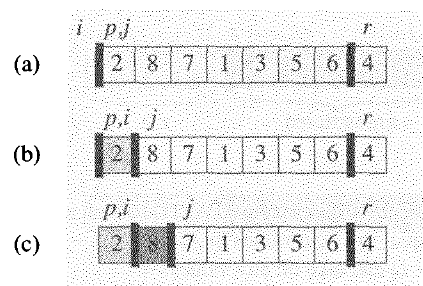
\includegraphics[scale=0.40]{img/trace_quicksort_1.png}}
                        \subfigure[Paso del 4 al 6]{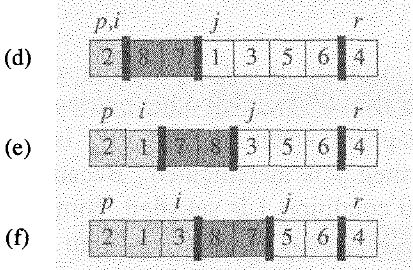
\includegraphics[scale=0.40]{img/trace_quicksort_2.png}}
                        \subfigure[Paso del 7 al 9]{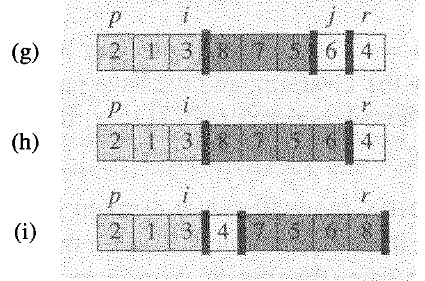
\includegraphics[scale=0.40]{img/trace_quicksort_3.png}}
                        \caption{Pasos del proceso de ordenamiento usando QuickSort} \label{fig:steps_quicksort}
                    \end{figure}
                    
                    \begin{enumerate}
                        \item \textbf{An\'{a}lisis}\\
                            \\
                            Para el algoritmo de QuickSort el tiempo de ejecuci\'{o}n depender\'{a} mucho de la forma en como los datos se encuentren, en este caso cuan balanceados los datos se presentan al inicio del ordenamiento.
                            
                            Por ello lo separaremos por mejor, peor y caso promedio:
                            
                            \textbf{Tiempo en el Peor Caso}:
                            
                            Este caso ocurre cuando se da una partici\'{o}n que genera n-1 elementos en un aubarray y 0 elementos en el otro subarray, adem\'{a}s esto ocurre en las dem\'{a}s llamadas recursivas, siendo un coste de partici\'{o}n de $\Theta(n) $, y la llamada del subarray de cero elementos ser\'{i}a $T(0) =  \Theta(1)$, siendo el tiempo de la llamada de recurrencia:
                            $$
                            T(n) = T(n-1) + T(0) + \Theta(n)
                            T(n) = T(n-1) + \Theta(n)
                            $$
                            
                            Resolviendo al recurrencia el tiempo tomado para el peor caso se produce un tiempo de $T(n) = O(n^2)$, es as\'{i} que es muy similar al caso del insertion sort, y esto ocurre cuando los elmentos de ingreso ya est\'{a}n completamente ordenados, en este caso insertion sort gana con un orden de $O(n)$.
                            
                            \textbf{Tiempo en el Mejor Caso}:
                            
                            Si se diera el caso de que los subarrays sean de tama\~{n}o no m\'{a}s de $n/2$, la recurrencia para el tiempo de ejecuci\'{o}n es: $T(n) = 2T(n/2) + \Theta(n)$ esta recurrencia tiene la soluci\'{o}n de $T(n) = O(nlgn)$.
                            
                            \textbf{Tiempo en el caso Promedio}:
                            
                            La clave para entender el coste promedio cercano al mejor caso es saber como se refleja el balanceo en la recurrencia.
                            
                            Si se da una partici\'{o}n en relaci\'{o}n de 9 a 1 partes se obtiene la siguiente recurrencia $T(n) \leq T(9n/10) + T(n/10) + cn $ este cuenta con el t\'{e}rmino oculto del coste de partici\'{o}n $\Theta n$ , como se observa en la figura, cada nivel al barre los n elementos tendr\'{i}a un coste de $cn$ hasta que sea alcanzado el primer nodo hoja dado en la profundidad $log_10(n) = \Theta(lg(n))$ a partir de aqu\'{i} cada nivel tendr\'{i}a a lo mucho un coste de $\leq c(n)$. La recursi\'{o}n termina en profundidad $log_(10/9)(n) = \Theta(lg(n))$ por ese motivo cualquiera sea el nivel siempre el coste ser\'{a} de $\Theta(lg(n))$ multiplicado por el coste del nivel $cn$ siendo asi un coste total de $\Theta(nlg(n))$. siempre y cuando exista almenos una divisi\'{o}n y sea constante durante todos los niveles del \'{a}rbol.
                            
                        \item \textbf{Implementaci\'{o}n C++}
                    
                            \lstinputlisting[language=C++, firstline=18, lastline=49, caption=quicksort.cpp]{code/quicksort.cpp}
                            
                        \item \textbf{Implementaci\'{o}n Python}\\
                    
                            \lstinputlisting[language=Python, firstline=8, lastline=47, caption=quicksort.py]{code/quicksort.py}
                    \end{enumerate}
                    
		         
		         \subsubsection{Selection Sort}
		            Una estrategia comun de ordenamiento es seleccionar el valor mas grande desde un array $A[0,n]$ e intercambiar su ubicación con el elemento que esta mas a la derecha $A[n-1]$. Este proceso se repite, subsecientemente, asi avanzar en cada pequeño rango sucesivo $A[0,n-1]$ hasta que A este ordenado, este es un caso del enfoque Greedy \cite{Heineman2008}.
		            
		            \begin{algorithm}[H]
                        \begin{algorithmic}[1]
                            \FOR{$i \gets 0$ to $N-1$}
                                \STATE $minIdx \gets i$
                                \FOR{$j \gets i+1$ to $N$}
                                    \IF{$A[j] < A[minIdx]$}
                                        \STATE $minIdx \gets j$ 
                                    \ENDIF
                                \ENDFOR
                                \STATE $A[j + 1] \gets key$
                            \ENDFOR
                        \end{algorithmic}
                        \caption{SELECTION-SORT(A)}
                        \label{alg:selection-sort}
                    \end{algorithm}
		            
		            \begin{enumerate}
                        \item \textbf{An\'{a}lisis}\\
                            Es el algoritmo de ordenamiento mas lento segun \cite{Heineman2008} en los algoritmos que nombra, requiere un tiempo $O(n^2)$ aun en el mejor caso, la lista totalmente ordenada, siempre seleccionando al elemento de mayor tamaño, tomando $n-1$ comparaciones, muchas de estas comparaciones son por desgaste, porque si un elemento es mas pequeño al segundo, es imposible ser el elemento de mayor tamaño, teniendo un desarrollo pobre al momento de continuar con las comparaciones.
                            
                            \begin{figure}[H]
                				\centering
                				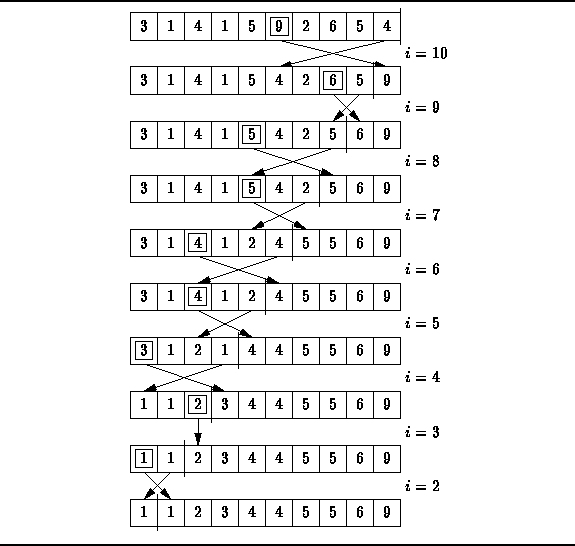
\includegraphics[scale=0.60]{img/selection_sort_img1.png}
                				\caption{Selection Sort en ejecución sobre una lista pequeña}
                				\label{fig:selection_sort_img1}
                			\end{figure}
                            
                        \item \textbf{Implementaci\'{o}n C++}
                    
                            \lstinputlisting[language=C++, firstline=11, lastline=35, caption=selectionSort.cpp]{code/selection.cpp}
                            
                            \item \textbf{Implementaci\'{o}n Python}\\
                    
                            \lstinputlisting[language=Python, firstline=9, lastline=20, caption=selectionSort.py]{code/selection.py}
                    \end{enumerate}
		    
		    
		    
		\subsection{Comparaci\'{o}n de tiempo de procesamiento}
		    
		        \subsubsection{Comparaci\'{o}n de dos lenguajes de programación por cada algoritmo} 
		        %% por cada algoritmo comparar en los dos lenguajes de programación
		        
		        Para todos los casos presentados en cada implementaci\'{o}n de los algoritmos, se ejecutaron utilizando los archivos generados anteriormente, iterando sobre todos ellos, luego en cada ejecucion de iteracion se realizo el calculo del tiempo en cada lenguaje de programacion dando como resultado un archivo con la cantidad de elementos y el tiempo de ejecución, en todos los casos se utilizó la libreria $matplotlib.pyplot$ de Python.
		        
		            \begin{enumerate}
		                \item \textbf{Bubble Sort: }
		                    Para calcular el tiempo del Bubble Sort en lenguaje C++ se utilizó la librería 
		                    $<$chrono$>$ que puede obtener un punto de tiempo que se representa en el tiempo ejecución, con el metodo now() podemos obtener los milisegundos exactos del inicio y fin del tiempo transcurrido
		                    
		                    \lstinputlisting[language=C++, firstline=1, lastline=12, caption=Ejecución C++ del Bubble Sort]{code/bubble_sort_tiempo.cpp}
		                
		                    En el caso del cálculo de tiempo en el lenguaje Python se utilizó la librería 'time' que gracias al metodo time.time() podemos obtener el tiempo de la ejecución en milisegundos
		                    
		                    \lstinputlisting[language=Python, firstline=1, lastline=10, caption=Ejecución Python del Bubble Sort]{code/bubble_sort_tiempo.py}
		                    
		                    La comparacion del tiempo de ejecucion del algoritmo Bubble Sort en los lenguajes C++ y Python, tiene como resultado una gran diferencia de tiempos con respecto a la cantidad de datos a ordenar, esto se debe a que el compilador de C++ es del propio sistema operativo y permite una ejecución directa de funciones, sin embargo Python tiene un compilador adaptado a una sintaxis resumida de funciones básicas del lenguaje maquina
		                    
		                    \begin{figure}[H]
                				\centering
                				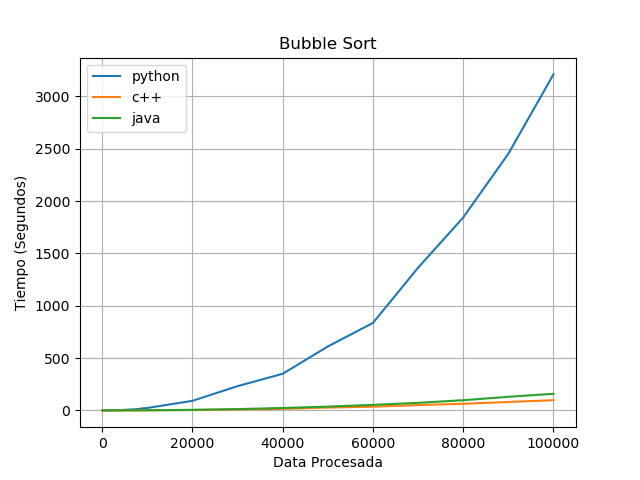
\includegraphics[scale=0.60]{img/bubble_sort_grafica.png}
                				\caption{Bubble Sort - Tiempo de Ejecución}
                				\label{fig:bubble_sort_grafica}
                			\end{figure}
		                    
		                \item \textbf{Counting Sort: }
		                Los tiempos de ejecución para las distintas dimensiones del arreglo se realizaron  en el orden de tiempo que demanda su coste O(n + k). Cabe resaltar que la ejecución del algoritmo en Python tiene tiempos más elevados que los ejecutados en C++.
                            
                            \lstinputlisting[language=C++, firstline=103, lastline=115, caption=Ejecucion C++ de CountingSort ]{code/counting.cpp}
                            
                            \lstinputlisting[language=Python, firstline=65, lastline=72, caption=Ejecucion Python de CountingSort]{code/counting.py}
                            
                            En la siguiente gráfica \ref{fig:counting_diagram} se muestra la comparación de los tiempos tomados para el algoritmo countingsort en 2 lenguajes Python y C++, donde se observa un comportamiento lineal cuando se ejecuto con C++ y una curva cercana a la lineal cuando se ejecutó con Python.
                            
                            \begin{figure}[H]
                                \centering
                                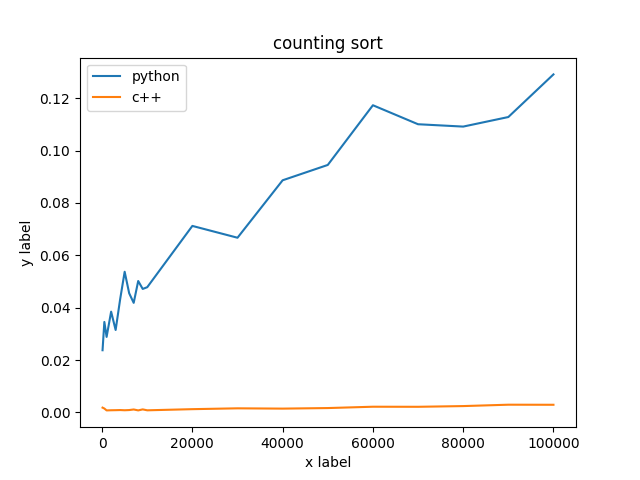
\includegraphics[scale=0.6]{img/counting_diagram.png}
                                \caption{CountingSort - Tiempo de Ejecución}
                                \label{fig:counting_diagram}
                            \end{figure}
		                \item \textbf{Heap Sort :}
                            Los tiempos de ejecución para los distintos tamanios de arreglo se realizaron  en el orden de tiempo que demanda su coste O(nlgn), además su costo es muy similar al del ordenamiento por quicksort.
                            
                            \lstinputlisting[language=C++, firstline=85, lastline=98, caption=Ejecucion C++ de Heapsort]{code/heapsort.cpp}
                            
                            A pesar de contar con un coste bajo para C++, heapsort en python tomaría un gran tiempo si la carga de datos es considerablemente enorme.
                            
                            \lstinputlisting[language=Python, firstline=72, lastline=78, caption=Ejecucion Python de Heapsort]{code/heapsort.py}
                            
                            En la siguiente gráfica \ref{fig:heapsort_diagram} se muestra la comparación de los tiempo tomados para el heapsort en 3 lenguajes Python, Java, y C++, donde se observa el crecimiento casi lineal del tiempo tomado por Python conforme la carga de datos crece, sin conocer ello y el orden de coste es importante pero también el lenguaje usado en la implementaci\'{o}n, Python al ser un lenguaje de alto nivel requiere el casting de sus funciones a funciones de librería base como C y poder recién realizar la ejecución.
                            
                            \begin{figure}[H]
                                \centering
                                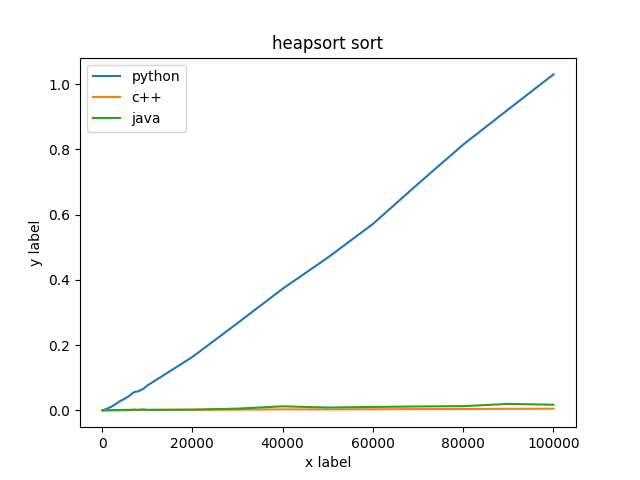
\includegraphics[scale=0.6]{img/heapsort_diagram.png}
                                \caption{Heapsort - Tiempo de Ejecución}
                                \label{fig:heapsort_diagram}
                            \end{figure}
		                
		                \item \textbf{Insertion Sort: }
		                    En el caso de la ejecución del Insertion Sort se utilizó para C++ la variable clock\textunderscore t que toma las pulsaciones de reloj del procesador luego pasado a segundos
		                    
		                    \lstinputlisting[language=C++, firstline=91, lastline=102, caption=Ejecucion C++ de Insertion Sort]{code/insertion.cpp}
		                    
		                    Igualmente en el caso de Python se toma la libreria $time$ para obtener la cantidad de tiempo de ejecución del algoritmo
		                    
		                    \lstinputlisting[language=Python, firstline=42, lastline=45, caption=Ejecucion Python de Insertion Sort]{code/insertion.py}
		                    
		                    Como resultado final se muestra la figura \ref{fig:insertion_diagram} la representación por cada lenguaje de programación ejecutado y medido, se incluyó Java solo con fines de comparacion ya que la finalidad solo era entre C++ y Python, demostrado ya en las pruebas anteriores en la generacion de los archivos se nota que el algoritmo hecho en C++ es mucho más rápido que en Python, ocurre porque la ejecución de C++ pasa directamente compilado para lenguaje máquina a diferencia de Python que es compilado en un lenguaje intermedio para luego recien pasar a lenguaje máquina.
		                    
		                    \begin{figure}[H]
                				\centering
                				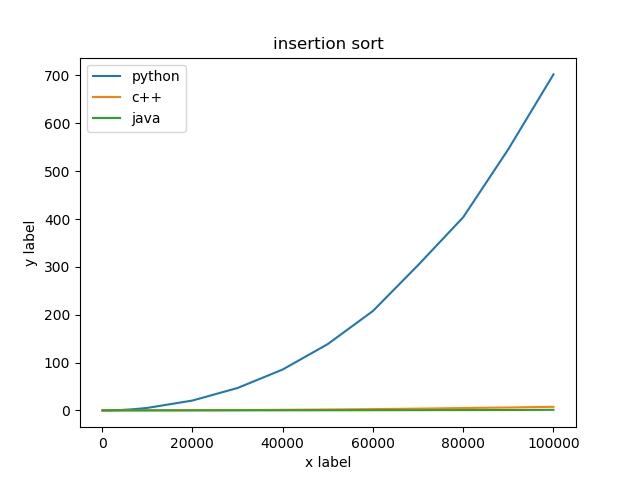
\includegraphics[scale=0.60]{img/insertion_diagram.png}
                				\caption{Insertion Sort - Tiempo de ejecución}
                				\label{fig:insertion_diagram}
                			\end{figure}
		                
		                \item \textbf{Merge Sort: }
		                Los tiempos de ejecución para las distintas dimensiones del arreglo se realizaron  en el orden de tiempo que demanda su coste O(nlogn). Cabe resaltar que la ejecución del algoritmo en Python tiene tiempos más elevados que los ejecutados en C++.
                            
                            \lstinputlisting[language=C++, firstline=133, lastline=147, caption=Ejecucion C++ de MergeSort ]{code/merge.cpp}
                            
                            \lstinputlisting[language=Python, firstline=81, lastline=88, caption=Ejecucion Python de MergeSort]{code/merge.py}
                            
                            En la siguiente gráfica \ref{fig:merge_diagram} se muestra la comparación de los tiempos tomados para el algoritmo mergesort en 2 lenguajes Python y C++, donde se observa un comportamiento lineal cuando se ejecuto con Python y una curva logarítmica cuando se ejecutó con C++.
                            
                            \begin{figure}[H]
                                \centering
                                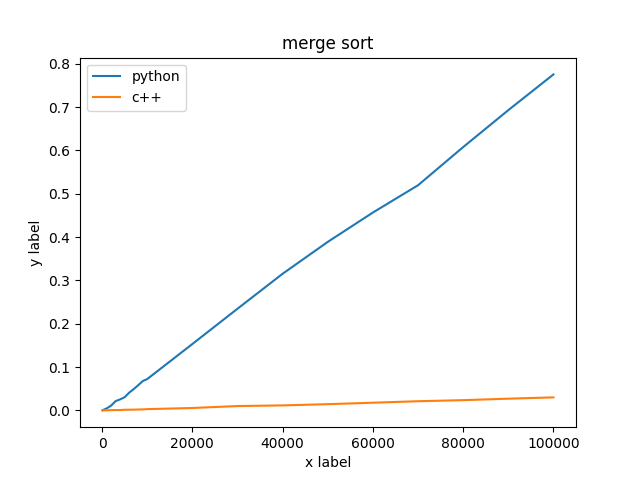
\includegraphics[scale=0.6]{img/merge_diagram.png}
                                \caption{MergeSort - Tiempo de Ejecución}
                                \label{fig:merge_diagram}
                            \end{figure}
		                \item \textbf{Quick Sort: }
                            El tiempo tomado para el quicksort fue el tomado de manera similar, para ello en el mejor caso podría comportarse muy similar al mergesort o heapsort $O(nlgn)$ pero en el peor caso podría comportarse como el selection sort $(n^2)$. El siguiente bloque de código muestra la captura de tiempo en C++.
                            
                            \lstinputlisting[language=C++, firstline=89, lastline=103, caption=Ejecucion C++ de Quicksort Sort]{code/quicksort.cpp}
                            
                            Para el caso de la implementaci\'{o}n en Python el crecimiento de datos es lineal pero con los últimos datos de tamanio mayor el tiempo se acentúa más, por ello se debe tener cuidado cuando se trabaje con una gran cantidad de datos en temas de ordenamiento, el lenguaje escogido puede ser muy sensitivo a la carga de datos como es el caso de Python. El siguiente bloque de código muestra la captura de tiempo de la llamada a quicksort en Python.
                            
                            \lstinputlisting[language=Python, firstline=67, lastline=73, caption=Ejecucion Python de Quicksort Sort]{code/quicksort.py}
                            
                            Finalmente se muestra la figura \ref{fig:quicksort_diagram} con la comparación en 3 lenguajes {Python, Java, y C++} en los tiempos de ejecución para una carga de datos des 100 hasta 100'000 datos a ordenar, para el caso de Python el crecimiento es exponencial a pesar de trabajar con algoritmos de ordenamiento bastante buenos en coste asintótico.
                            
                            \begin{figure}[H]
                                \centering
                                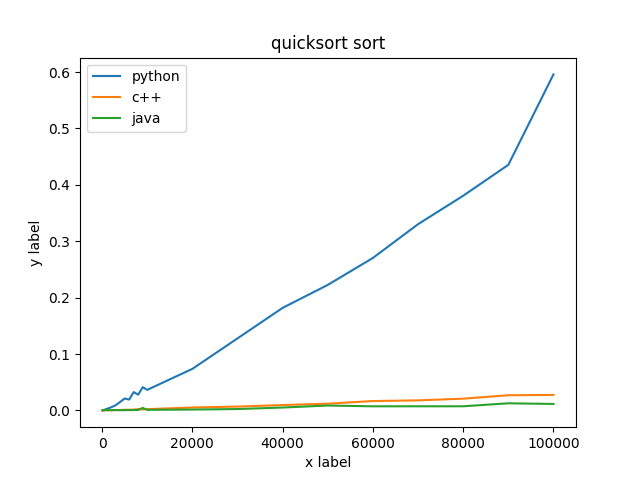
\includegraphics[scale=0.60]{img/quicksort_diagram.png}
                                \caption{Selection Sort - Tiempo de ejecución}
                                \label{fig:quicksort_diagram}
                            \end{figure}
		                
		                \item \textbf{Selection Sort: }
		                    En el caso de la ejecución del Selection Sort se utilizó para C++ la variable clock\textunderscore t que toma las pulsaciones de reloj del procesador luego pasado a segundos
		                    
		                    \lstinputlisting[language=C++, firstline=92, lastline=101, caption=Ejecucion C++ de Selection Sort]{code/selection.cpp}
		                    
		                    Igualmente en el caso de Python se toma la libreria $time$ para obtener la cantidad de tiempo de ejecución del algoritmo
		                    
		                    \lstinputlisting[language=Python, firstline=39, lastline=42, caption=Ejecucion Python de Selection Sort]{code/selection.py}
		                    
		                    Como resultado final se muestra la figura \ref{fig:selection_diagram} la representación por cada lenguaje de programación ejecutado y medido, se incluyó Java solo con fines de comparación ya que la finalidad solo era entre C++ y Python, demostrado ya en las pruebas anteriores en la generacion de los archivos se nota que el algoritmo hecho en C++ es mucho más rápido que en Python, ocurre porque la ejecución de C++ pasa directamente compilado para lenguaje máquina a diferencia de Python que es compilado en un lenguaje intermedio para luego recien pasar a lenguaje máquina.
		                    
		                    \begin{figure}[H]
                				\centering
                				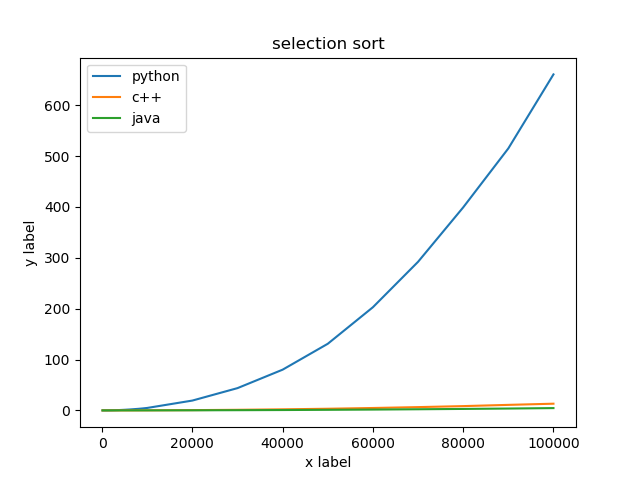
\includegraphics[scale=0.60]{img/selection_diagram.png}
                				\caption{Selection Sort - Tiempo de ejecución}
                				\label{fig:selection_diagram}
                			\end{figure}
		                    
		                
		            \end{enumerate}
		        
		        \subsubsection{Comparación de tiempo de procesamiento de todos los algoritmos implementados en cada lenguaje de programación}
		            Finalizando la revisión de los algoritmos directamente en sus implementaciones en C++ y Python, se observa que desde el análisis en cada uno de los algoritmos presentados se puede observar como el algoritmo mas ineficiente a Bubble Sort y los mas eficientes a los que están con tiempo logarítmico (HeapSort, MergeSort, QuickSort) incluso tomar a Coounting Sort en estos casos pero su tendencia solo aplica a este tipo de ordenamiento con números mayores a 0 y enteros además de la dependencia del consumo de memoria.
		            \\
		            
		            Respectivamente en la Figura \ref{fig:sort-algorithms-cpp} de C++ se observa la gráfica menos notoria en algunos algoritmos pesados como Insertion Sort, por el resultado en bajo tiempo respecto a la Figura \ref{fig:sort-algorithms-python} que muestra mayor notoriedad en los algoritmos ya que sus resultados fueron mas extensos respecto al lenguaje C++.  
		        
		            \begin{figure}[H]
        				\centering
        				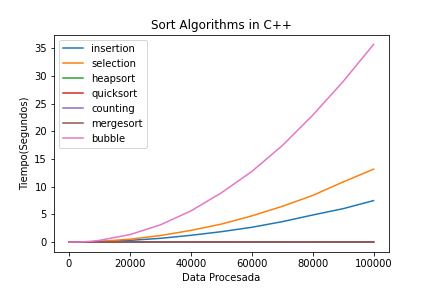
\includegraphics[scale=0.60]{img/sort-algorithms-cpp.png}
        				\caption{Algoritmos de Ordenamiento implementados en C++}
        				\label{fig:sort-algorithms-cpp}
                	\end{figure}
                			
                	\begin{figure}[H]
        				\centering
        				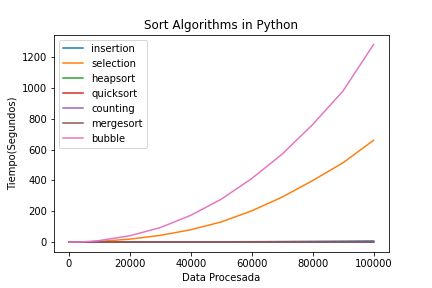
\includegraphics[scale=0.60]{img/sort-algorithms-python.png}
        				\caption{Algoritmos de Ordenamiento implementados en Python}
        				\label{fig:sort-algorithms-python}
        			\end{figure}
        			
        			En conclusión cada uno de los algoritmos presentados cumplen un mismo objetivo en ordenar los elementos de un arreglo con diferentes enfoques de resolución y ejecución, mostrando tanto sus beneficios como dificultades, siempre realizando la comparación con el peor caso y la revisión en tiempos de ejecución nos mostro que tan factible es elegir un algoritmo respecto a otro.
        			
		        %% solamente dos graficos para la comparacion.
		        %\clearpage
    
    \newpage
    
	\bibliographystyle{ieeetr}
    % bib stuff
    \nocite{*}
    \bibliography{biblio}
	%\bibliographystyle{apalike}
	%\bibliographystyle{IEEEtranN}
	%\bibliography{bibliography}
	
	\newpage
	
	\lstlistoflistings	
	
\end{document}